\documentclass[tikz, border = 10pt]{standalone}

\usepackage{newpxtext,newpxmath}   % /upbeta
%\usepackage{fouriernc}            % /otherbeta
\usepackage{amsmath}
\renewcommand{\familydefault}{\sfdefault}
\usepackage{mathastext}

\usetikzlibrary{positioning, quotes, calc, math, arrows.meta, bending, shapes, backgrounds}

\tikzset{
every edge quotes/.style = {fill = white},
every node/.style = {scale = 1.1},
manifest/.style = {rectangle, draw, thin, inner sep = 3pt, minimum width = 1cm,
   minimum height = .85cm, align = center},
latent/.style = {ellipse, draw, thin, inner sep = 3pt, minimum width = 1cm,
   minimum height = .85cm},
residual1/.style = {circle, draw, thin, minimum size = 5mm, inner sep = 1pt},
residual2/.style = {rectangle, minimum width = 0.5pt, minimum height = 1.5mm,
   inner sep = 0pt, outer sep = 0mm},
regression/.style = {-{Stealth[length = 1.5mm]}, thin, shorten > = 1pt, 
   inner sep = 1.5pt, outer sep = 0mm},
covariance/.style={{Stealth[length = 1.5mm]}-{Stealth[length = 1.5mm]}, thin,
   shorten > = 1pt, shorten < = 1pt, inner sep = 1.5pt},
variance/.style={{Stealth[length = 1mm]}-{Stealth[length = 1mm]}, thin,
   shorten > = 1pt, shorten < = 1pt, inner sep = 1pt},
interaction/.style = {-{Stealth[sep = 1pt, length = 1.5mm] . Circle[length = 4pt]},
   thin, shorten > = -2pt},
constant/.style = {draw, thin, inner sep = 1pt, regular polygon,
   regular polygon sides = 3, minimum size = 5mm},
group/.style = {rectangle, inner sep = 2pt, minimum width = 15mm, minimum height = 5mm, 
   align = center}
}

\begin{document}
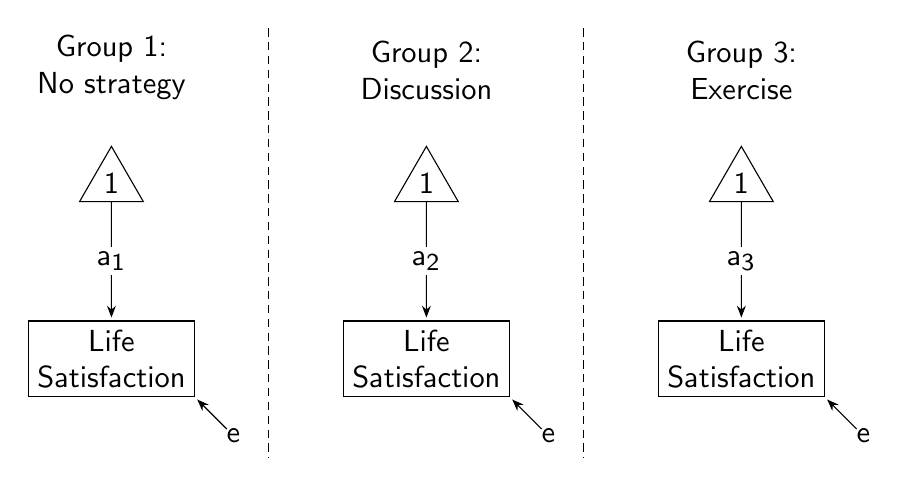
\begin{tikzpicture}

\newcommand\gap{2}            % separation between dependents
\def\list{1/No strategy, 2/Discussion, 3/Exercise}

\foreach \i/\j in \list {
   %% Dependent
   \tikzmath{\x = (2 + \gap) * (\i - 1);}        % x-coord for Dependents
   \node [manifest] (y\i) at (\x, 0) {Life\\Satisfaction};

   %% Residuals
   \node [residual2] (e\i) [below right = 4mm and 4mm of y\i] {e};
   \path [regression] (e\i) edge (y\i.south east);

   %% Means
   \node [constant] (const\i) [above = 1.5cm of y\i] {1};
   \path [regression] (const\i) edge ["a$_\i$"] (y\i);

   %% Groups
   \node [group] (gp\i) [above = 0.5cm of const\i] {Group \i:\\\j};
}

%% Separators
\foreach \i in {1,2} {
   \tikzmath {\j = int(\i + 1);}
   \coordinate (M) at ($(y\i)!0.5!(y\j)$);
   \draw [style = densely dashed, thin] ($(M)!4.2cm!270:(y\i)$) -- ($(M)!1.25cm!90:(y\i)$);
}

\end{tikzpicture}
\end{document}